% Created 2015-11-03 Tue 05:46
\documentclass[presentation]{beamer}
\usepackage[utf8]{inputenc}
\usepackage[T1]{fontenc}
\usepackage{fixltx2e}
\usepackage{graphicx}
\usepackage{grffile}
\usepackage{longtable}
\usepackage{wrapfig}
\usepackage{rotating}
\usepackage[normalem]{ulem}
\usepackage{amsmath}
\usepackage{textcomp}
\usepackage{amssymb}
\usepackage{capt-of}
\usepackage{hyperref}
\usetheme{default}
\usecolortheme{beaver}
\author{Ustun Ozgur}
\date{2015-11-03 Tue}
\title{Flux}
\hypersetup{
 pdfauthor={Ustun Ozgur},
 pdftitle={Flux},
 pdfkeywords={},
 pdfsubject={},
 pdfcreator={Emacs 24.4.1 (Org mode 8.3.2)},
 pdflang={English}}
\begin{document}

\maketitle


\begin{frame}[label={sec:orgheadline1}]{Flux}
\begin{itemize}
\item open sourced by Facebook
\item not a library, a technique like MVC
\item suitable for bigger applications
\end{itemize}
\end{frame}

\begin{frame}[label={sec:orgheadline2}]{When is Flux a good idea?}
\begin{itemize}
\item Too deep level in React hiearchy
\item Need to pass props to the bottom too much
\item Two components not having a single parent, but want to sync state
\end{itemize}
\end{frame}


\begin{frame}[label={sec:orgheadline3}]{Stores}
\begin{itemize}
\item Enclose the domain logic
\item Act as event emitters
\item Emits a change event whenever it changes
\item Simple version, not Flux: No actions
\item React component intercepts the events, forwards them to store
\item React component subscribe to store events
\item React component syncs its state with store
\end{itemize}
\end{frame}

\begin{frame}[label={sec:orgheadline4}]{Actions}
\begin{itemize}
\item As apps get big, react component should not call store directly
\item Instead a level of indirection
\item React components intercept events
\item Forward them to dispatcher as events
\end{itemize}
\end{frame}

\begin{frame}[label={sec:orgheadline5}]{Dispatcher}
\begin{itemize}
\item Dispatcher broadcasts events to all stores
\item Stores decide which events they are interested in
\item They decide accordingly and emit a change event
\item React components sync accordingly
\end{itemize}
\end{frame}

\begin{frame}[label={sec:orgheadline6}]{Flux Architecture (1/3)}
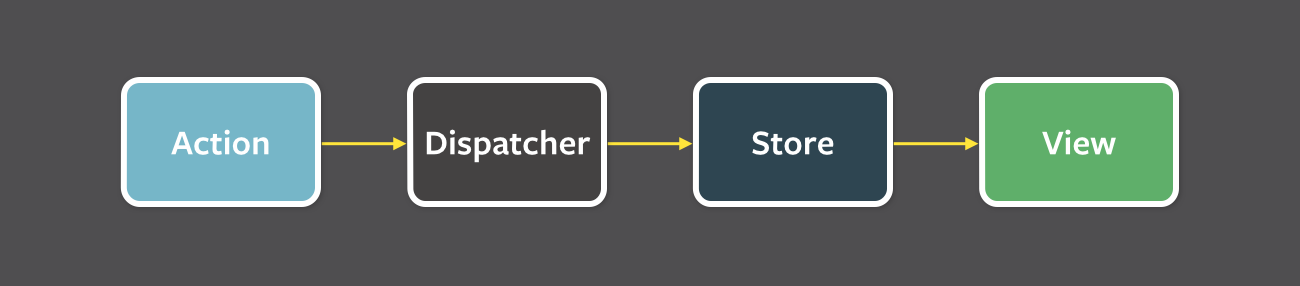
\includegraphics[width=.9\linewidth]{./flux1.png}
\end{frame}



\begin{frame}[label={sec:orgheadline7}]{Flux Architecture (2/3)}
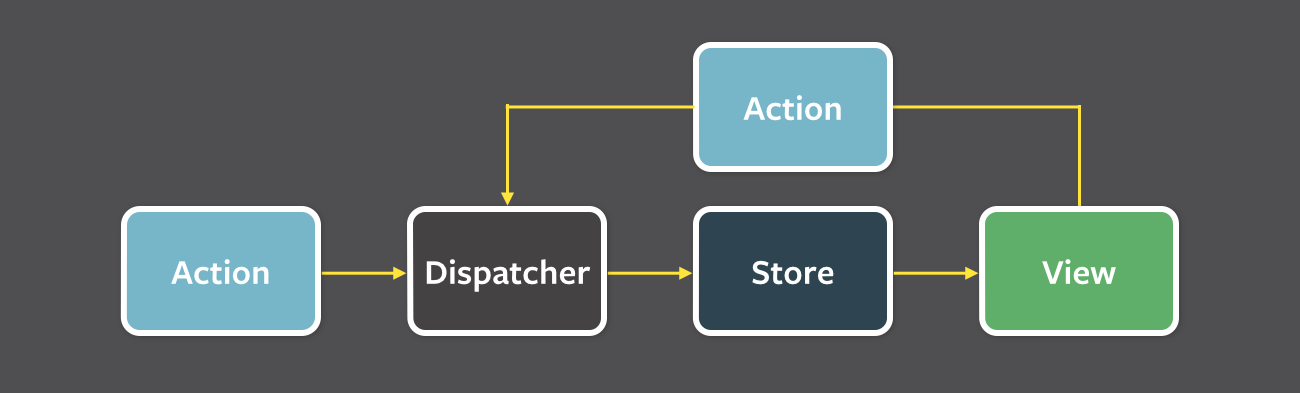
\includegraphics[width=.9\linewidth]{./flux2.png}
\end{frame}
\begin{frame}[label={sec:orgheadline8}]{Flux Architecture (3/3)}
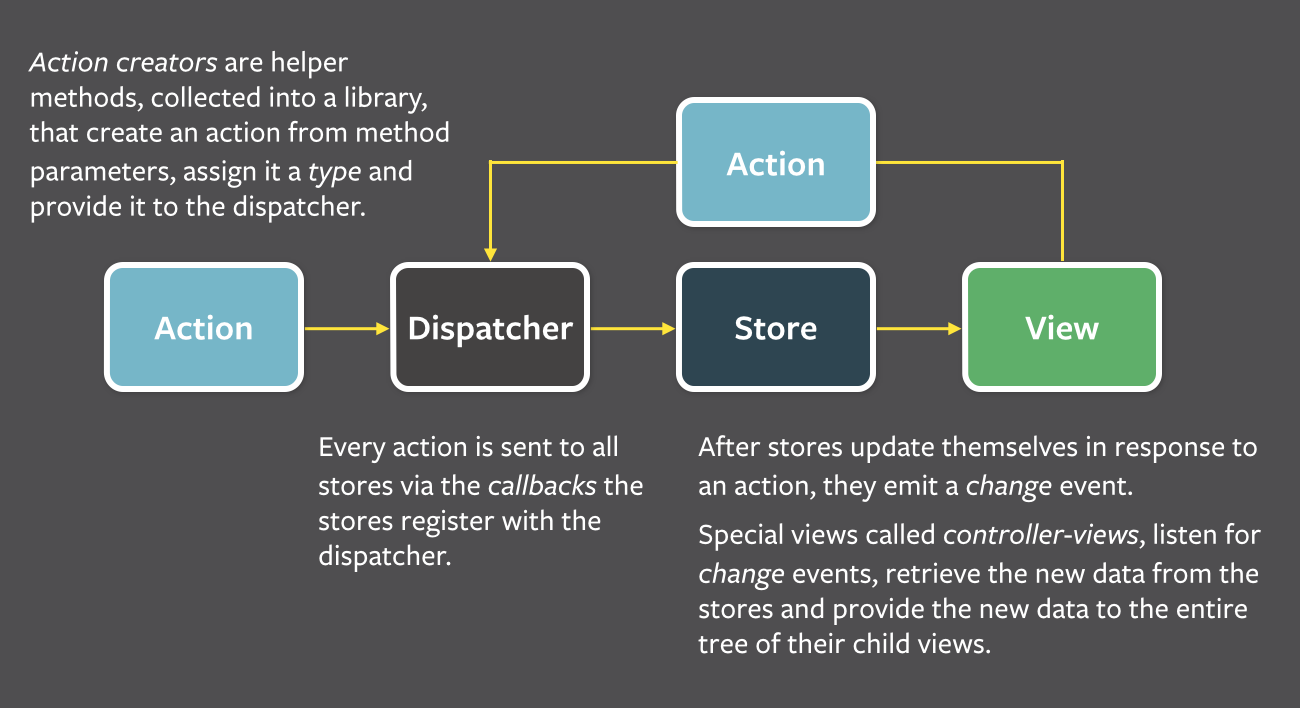
\includegraphics[width=.9\linewidth]{./flux3.png}
\end{frame}
\begin{frame}[label={sec:orgheadline9}]{Detail}
\begin{itemize}
\item \emph{Demo}
\end{itemize}
\end{frame}
\end{document}
